\subsection{Seed Synthesizer}

To synthesize seed JavaScript programs, we implement two different
synthesizers: \textit{non-recursive synthesizer} and \textit{built-in function
synthesizer}.
\newline

\subsubsection{Non-Recursive Synthesizer}

The main goal of the non-recursive synthesizer is to cover various cases of
syntax.  It consists of two steps: 1) to find the shortest string for each
non-terminal and 2) to synthesize JavaScript programs using the pre-calculated
shortest strings.  While we support various extended rules in grammar of
ECMAScript such as parametric non-terminals, conditional alternatives, and
various special terminal symbols, we focus on simple terminals and non-terminals
in this section for the brevity.

\begin{algorithm}[t]
  \caption{Worklist-based Shortest String}
  \label{alg:short-string}
  \DontPrintSemicolon
  \SetKwProg{Fn}{Function}{:}{}
  \SetKwFunction{shortestStrings}{shortestStrings}
  \SetKwFunction{update}{update}
  \SetKwFunction{propagate}{propagate}
  \KwIn{$\ruleset$ - syntax reduction rules}
  \KwOut{$M$ - map from non-terminals to shortest strings}
  \Fn{\shortestStrings{$\ruleset$}} {
    $M = \varnothing, \worklist = \text{a queue that consists of}\ \ruleset$\;
    \While{$\worklist \neq \varnothing$} {
      $\text{pop}\ (A, \alpha) \gets \worklist$\;
      \lIf{$\update(A, \alpha)$} {
        $\propagate(\worklist, \ruleset, A)$
      }
    }
  }
  \Fn{\update{$A, \alpha$}} {
    $str = \text{an empty string}$\;
    \ForAll{$s \in \alpha$} {
      \lIf{$s\ \text{is a terminal}\ t$} {
        $str = str + t$
      }
      \ElseIf{$s\ \text{is a non-terminal}\ A \wedge A \in M$} {
        $str = str + M[A]$
      }
      \lElse {
        \Return false
      }
    }
    \lIf{$\exists M[A] \wedge \norm{str} \geq \norm{M[A]}$} {
      \Return false
    }
    $M[A] = str$\;
    \Return true\;
  }
  \Fn{\propagate{$\worklist, \ruleset, A$}} {
    \ForAll{$(A', \alpha') \in \ruleset$} {
      \lIf{$A \in \alpha'$} {
        $\text{push}\ (A', \alpha') \rightarrow \worklist$
      }
    }
  }
\end{algorithm}

For the first step, we find the shortest string for each non-terminal via the
\textsf{shortestStrings} function described in Algorithm~\ref{alg:short-string}.
We modifies the algorithm introduced by McKenize~\cite{cfg-gen} to find the
shortest string instead of a random string.  It takes syntax reduction rules
$\ruleset$, which is a set of pairs of non-terminals and alternatives and
returns a map $M$ from non-terminals to their shortest strings.  It utilizes a
worklist $W$, which is a queue structure that includes syntax reduction rules
that affected by updated non-terminals.  The function initializes the worklist
$W$ with all syntax reduction rules $\ruleset$.  Then, it extracts a syntax
reduction rule $(A, \alpha)$, updates the map $M$ via the \textsf{update}
function, and propagate updated information via the \textsf{propagate} function.
The \textsf{update} function checks whether the given alternative $\alpha$ of
the non-terminal $A$ can derive a string shorter than the current shortest one
based on the current map $M$.  If it is possible, it stores the pair the
non-terminal $A$ and the newly found shortest string in the map $M$ and invokes
the \textsf{propagate} function.  The \textsf{propagate} function finds all
syntax reduction rules whose alternatives contains the updated non-terminal $A$
and inserts them into the worklist $W$.  The \textsf{shortestStrings} function
repeats this process until the worklist $W$ becomes empty.

\begin{algorithm}[t]
  \caption{Non-Recursive Synthesize}
  \label{alg:non-rec-synthesize}
  \DontPrintSemicolon
  \SetKwProg{Fn}{Function}{:}{}
  \SetKwFunction{nonRecSynthesize}{nonRecSynthesize}
  \SetKwFunction{getProd}{getProd}
  \SetKwFunction{getAlt}{getAlt}
  \KwIn{$\ruleset$ - syntax reduction rules, $S$ - start symbol}
  \KwOut{$D$ - set of strings derivable from $S$}
  \SetKwBlock{Begin}{function}{end function}
  \Fn{\nonRecSynthesize{$\ruleset, S$}} {
    $V = \varnothing, M = \shortestStrings(\ruleset)$\;
    \Return $\getProd(M, V, \ruleset, S)$\;
  }
  \Fn{\getProd{$M, V, \ruleset, A$}} {
    \lIf{$A \in V$} {
      \Return $\{ M[A] \}$
    }
    $D = \varnothing, V = V \cup \{ A \}$\;
    \ForAll{$(A', \alpha) \in \ruleset\ \text{s.t.}\ A' = A$} {
      $D = D \cup \getAlt(M, V, \ruleset, A, \alpha)$\;
    }
    \Return $D$\;
  }
  \Fn{\getAlt{$M, V, \ruleset, A, \alpha$}} {
    $L = \text{an empty list}$\;
    \ForAll{$s \in \alpha$} {
      \If{$s\ \text{is a terminal}\ t$} {
        $\text{append}\ (\{ t \}, t) \rightarrow L$\;
      }
      \ElseIf{$s\ \text{is a non-terminal}\ A'$} {
        $\text{append}\ (\getProd(M, V, \ruleset, A'), M[A])
        \rightarrow L$\;
      }
    }
    $D =$ point-wise concatenation of first elements of pairs in $L$ and use
    second elements for short cases.\;
    \Return $D$\;
  }
\end{algorithm}

After finding shortest strings for non-terminals, we synthesize programs via the
\textsf{nonRecSynthesize} function.  It takes syntax reduction rules $\ruleset$
and a start symbol $S$.  To reduce the number of redundant syntax elements, it
keeps the visited set $V$ of non-terminals and utilizes the map $M$ produced by
the \textsf{shortestStrings} function.  For the first visit with a non-terminal
$A$, The \textsf{getProd} function takes and returns unions of sets of strings
generated by invoking the \textsf{getAlt} algorithm with alternatives of the
non-terminal $A$.  However, if the already visited non-terminal $A$ is passed,
it returns the single shortest string $M[A]$.  The \textsf{getAlt} takes a
non-terminal $A$ with an alternative $\alpha$ and returns a set of strings
derivable from $\alpha$ via point-wise concatenation of strings derived by
symbols of $\alpha$.  If the numbers of strings derived by symbols are
different, the shortest strings are used to fill out the short cases.

\begin{figure}[t]
  \centering
  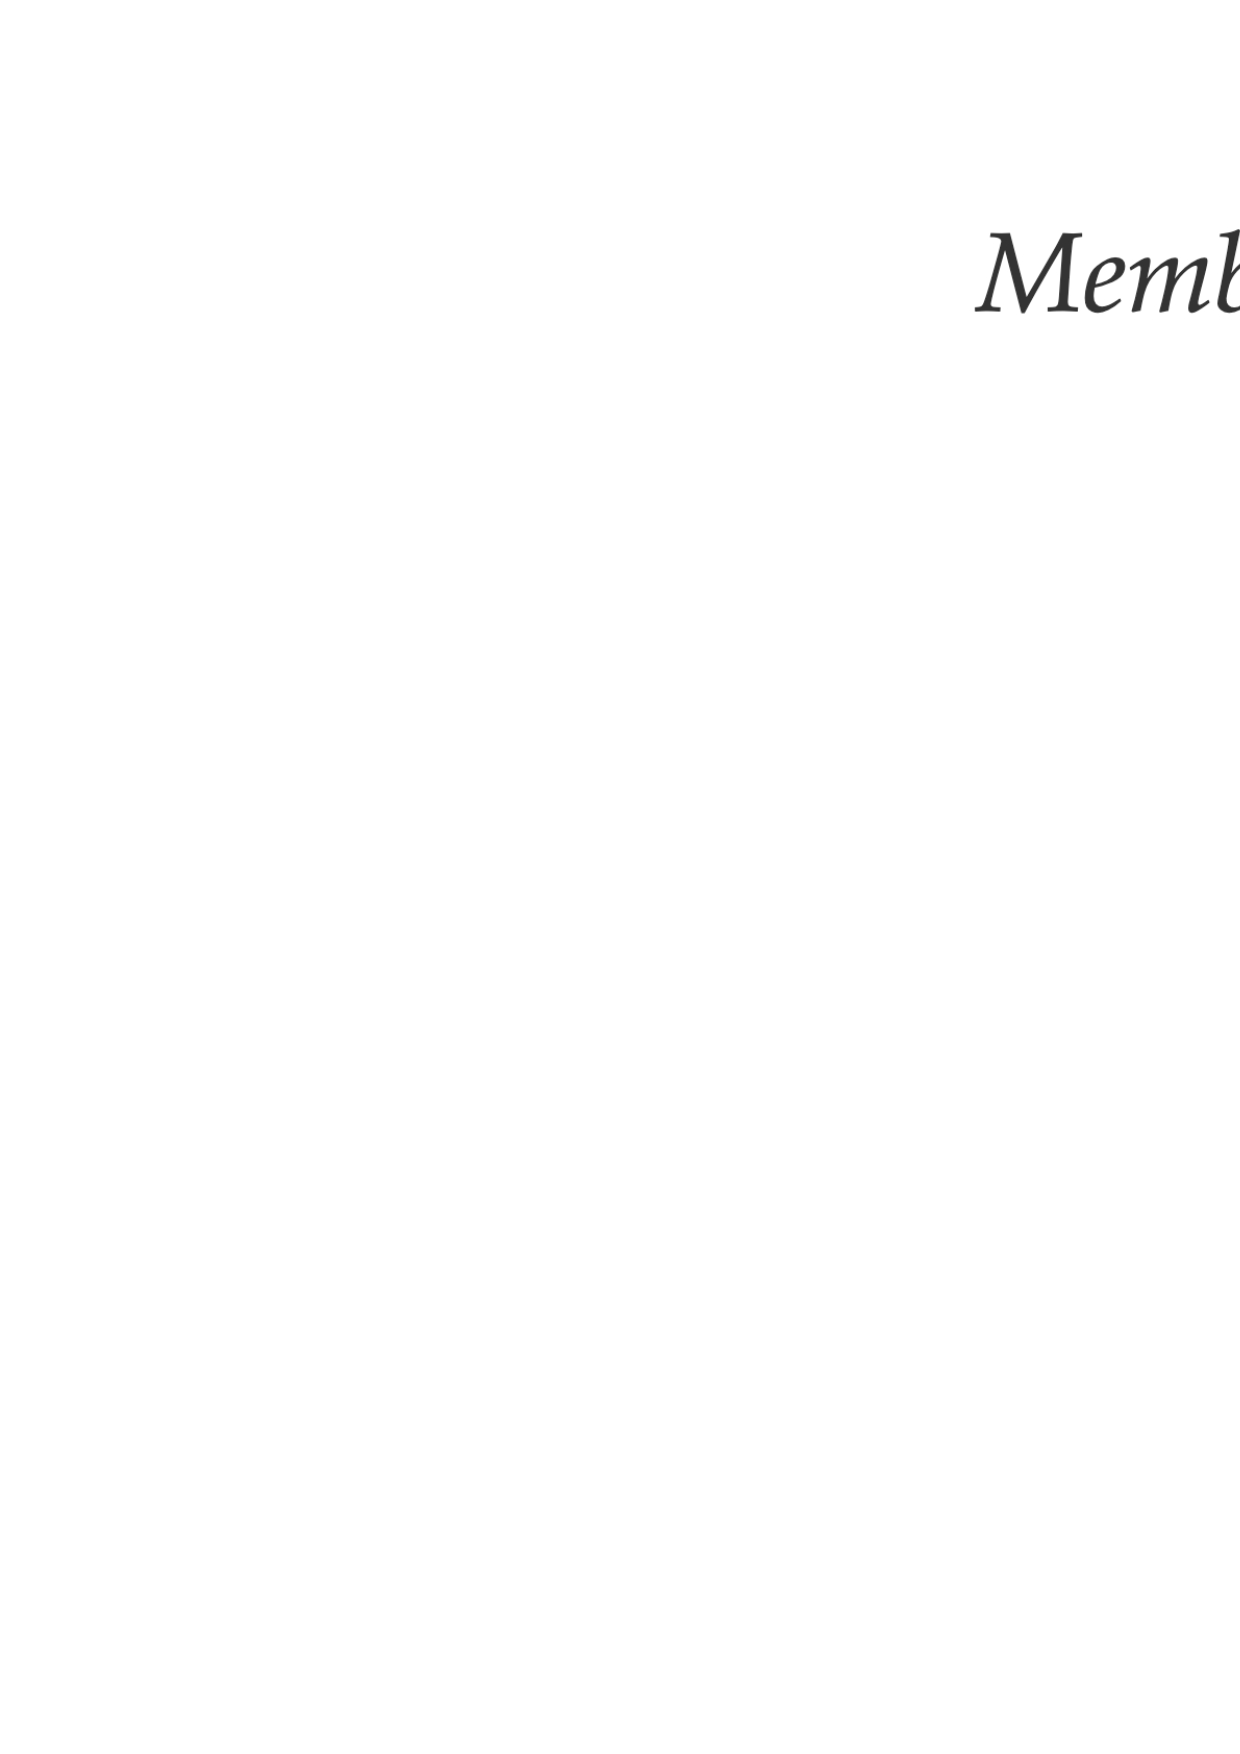
\includegraphics[width=0.32\textwidth]{img/syntax-member.pdf}
  \caption{The \textit{MemberExpression} production in ES11}
  \label{fig:prod-example}
  \vspace*{-1em}
\end{figure}

For example, Figure~\ref{fig:prod-example} shows the simplified
\textit{MemberExpression} production in ES11.  For the first step, we find
the shortest string for each non-terminal: \code{()} for \textit{Arguments} and
\code{x} for other non-terminals.  In the next step, we synthesize the strings
derivable from \textit{MemberExpression}.  The first alternative consists of a
single non-terminal \textit{PrimaryExpression} and it is the first time to visit
it.  Thus, it generates all cases of \textit{PrimaryExpression}.  The fourth
alternative consists of one terminal \code{new} and two non-terminals
\textit{MemberExpression} and \textit{Arguments}.  The \textit{MemberExpression}
is already visited thus it generates a single shortest string \code{x} but it is
the first time to visit \textit{Arguments}.  It generates all cases: \code{()},
\code{(x)}, \code{(...x)}, and \code{(x,)}.  However, the numbers of strings for
its symbols are different with each other.  To match the number of strings, we
fill out the short cases with terminal itself for \code{new} and the shortest
string \code{x} for \textit{MemberExpression} as follows:

\begin{figure}[H]
  \centering
  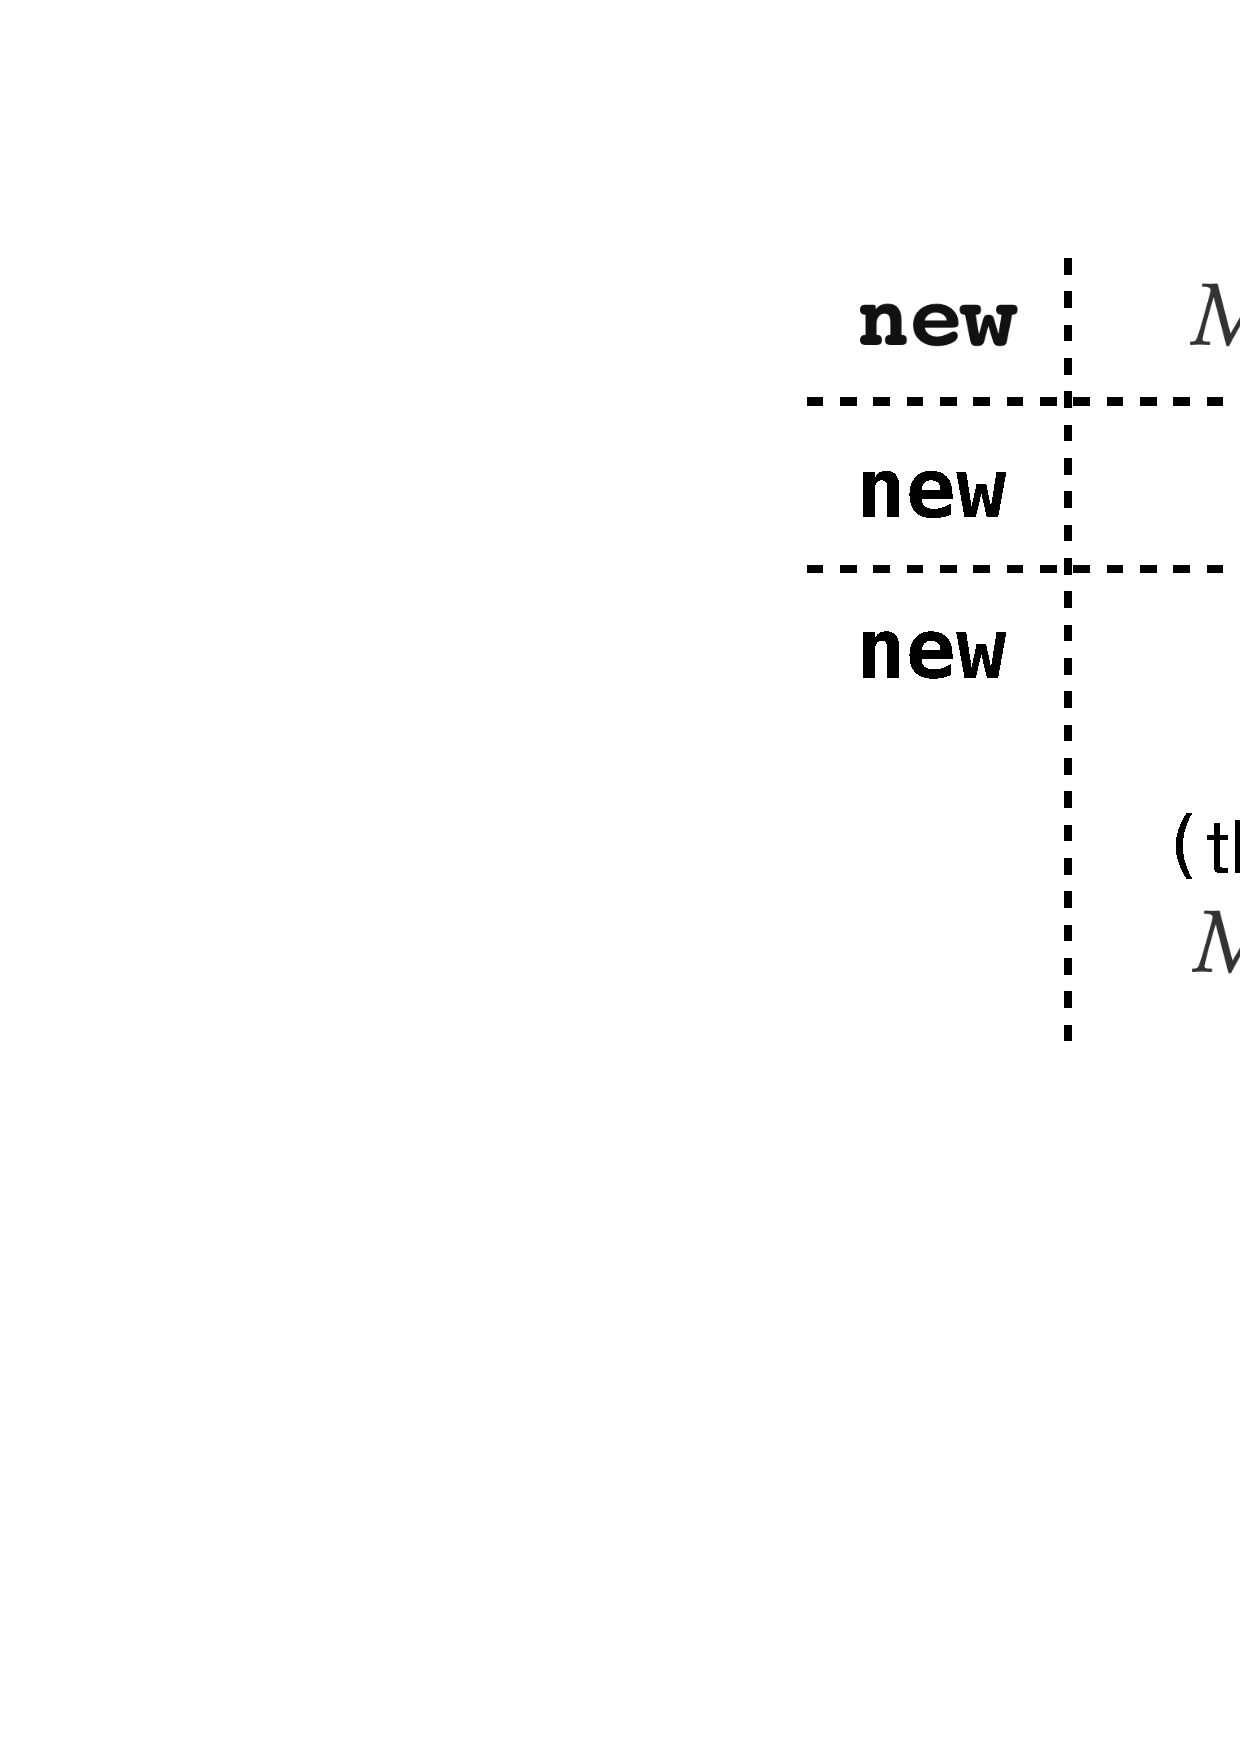
\includegraphics[width=0.48\textwidth]{img/member-example.pdf}
\end{figure}


\subsubsection{Built-in Function Synthesizer}

JavaScript includes various kinds of built-in functions to provide more
functionalities related to primitive values and built-in objects.  To cover
their semantics, we extract information for each built-in function from
mechanized ECMAScript and synthesize JavaScript programs that invoke built-in
functions.  We utilize \code{Function.prototype.call} function to invoke
built-in functions to easily handle the \code{this} object in \textsf{Program
Mutator}.  In this step, we pass a corresponding object or \code{null} as the
\code{this} object in default.  To consider optional and variable arguments, we
synthesize function calls with various number of arguments.  Moreover, we
consider not only built-in functions but also built-in constructors with the
\code{new} keyword.

\begin{figure}[H]
  \centering
  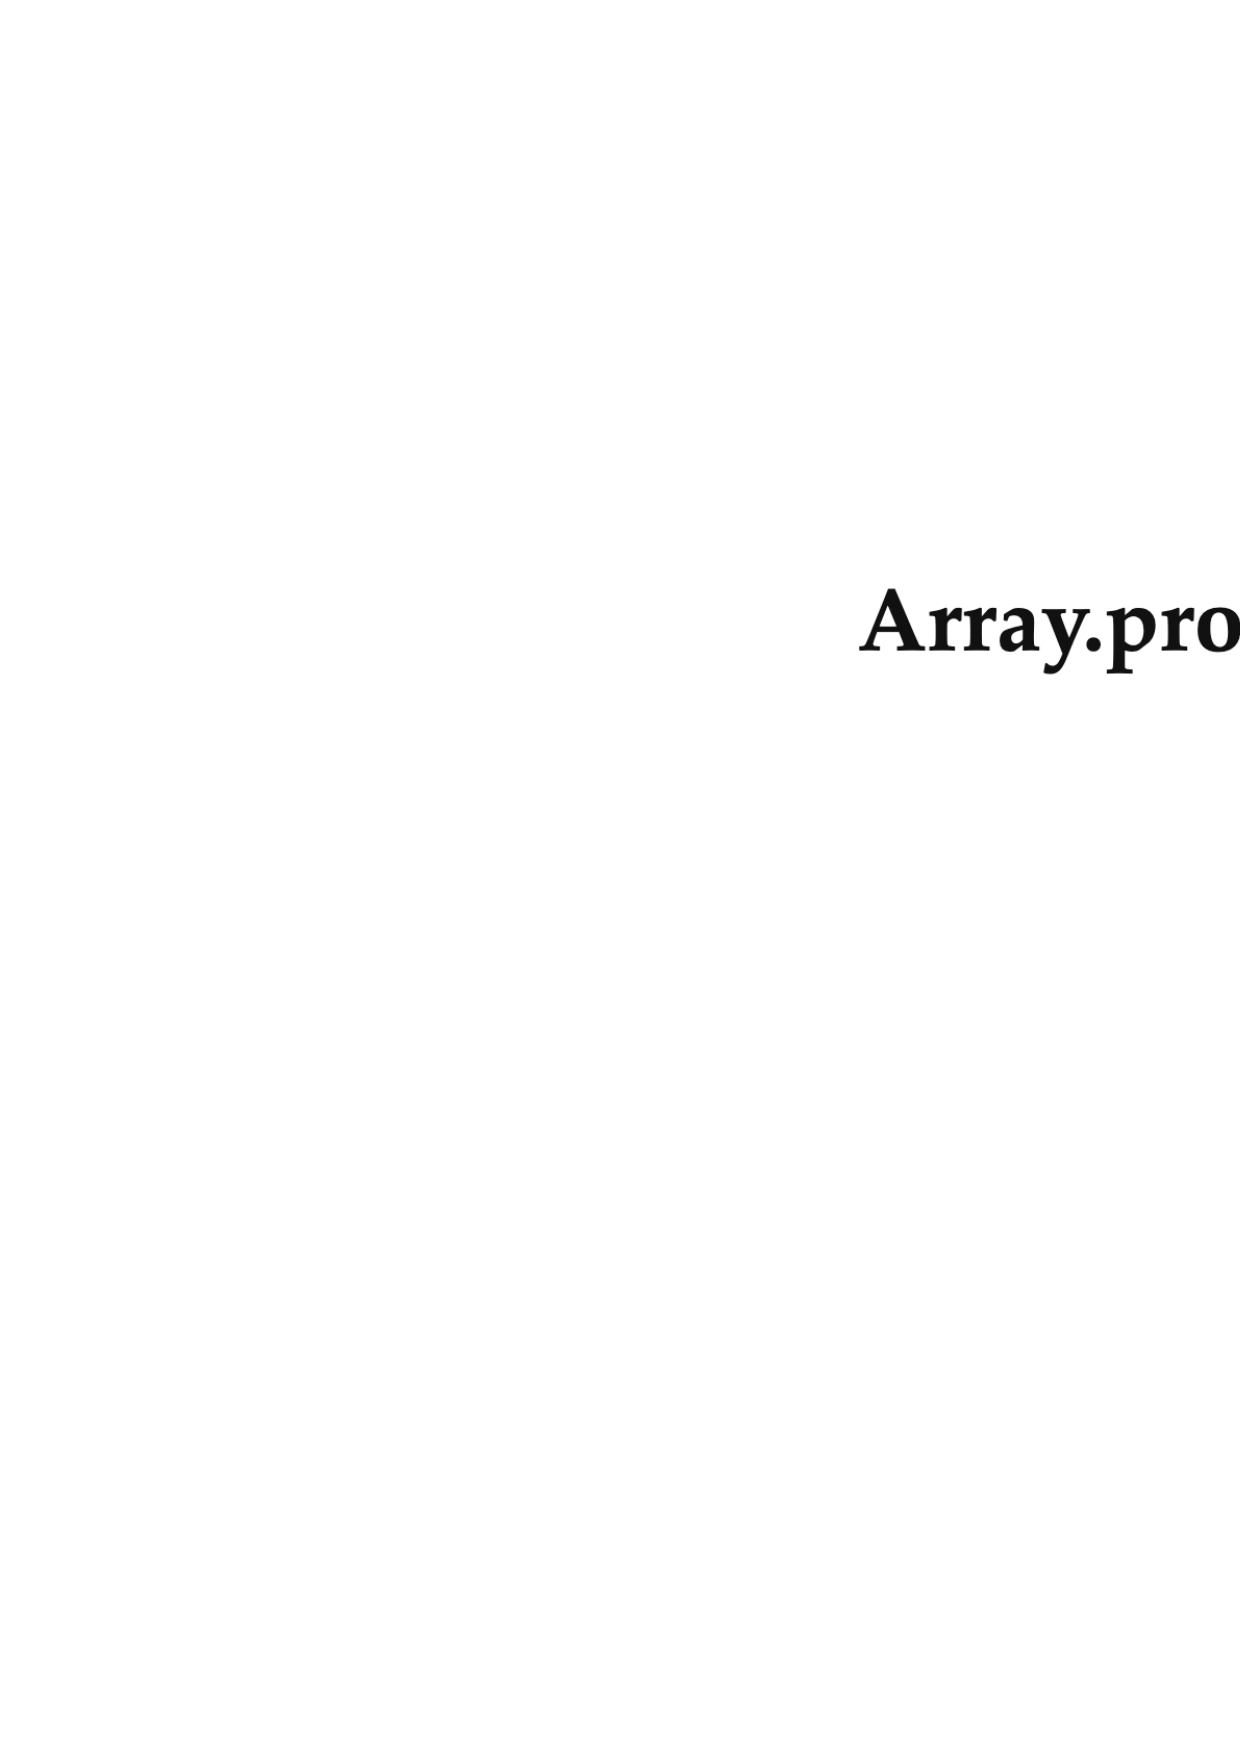
\includegraphics[width=0.4\textwidth]{img/array-indexof.pdf}
\end{figure}

For example, consider the above \code{Array.prototype.indexOf} function for
JavaScript array objects.  It takes one parameter \textit{searchElement} that
denotes the element we want to search and one more optional parameter
\textit{fromIndex} to change the searching scope.  Thus, the synthesizer passes
one or two arguments with an array object or \code{null} as the \code{this}
object as follows:
\begin{lstlisting}[style=myJSstyle]
Array.prototype.indexOf.call(new Array(), 0);
Array.prototype.indexOf.call(new Array(), 0, 0);
Array.prototype.indexOf.call(null, 0);
Array.prototype.indexOf.call(null, 0, 0);
\end{lstlisting}
Moreover, \code{Array} itself is also not only a built-in function but also
a built-in constructor with an optional single argument or variable arguments.
Thus, we synthesize the following six programs for \code{Array}:
\begin{lstlisting}[style=myJSstyle]
Array();      Array(0);      Array(0, 0);
new Array();  new Array(0);  new Array(0, 0);
\end{lstlisting}
